
\chapter{Análisis de sensibilidad por moneyness y vencimiento}
\label{app:sensibilidad-moneyness-vencimiento}

Este apéndice desarrolla, en formato operativo, la sensibilidad del error por regiones de superficie. Se apoya en las vistas de \emph{Diagnosis}, donde se integran tres gráficos clave: \emph{Residual Heatmap}, \emph{Error by Maturity} y \emph{Error by Moneyness}. El objetivo es localizar zonas de mayor fragilidad para valoración y control de riesgos, no solo reportar un error promedio. Funciona como ampliación técnica de la Sección~\ref{sec:aplicaciones-operativas}.

\begin{figure}[htbp]
\centering
\begin{minipage}{0.49\textwidth}
\centering
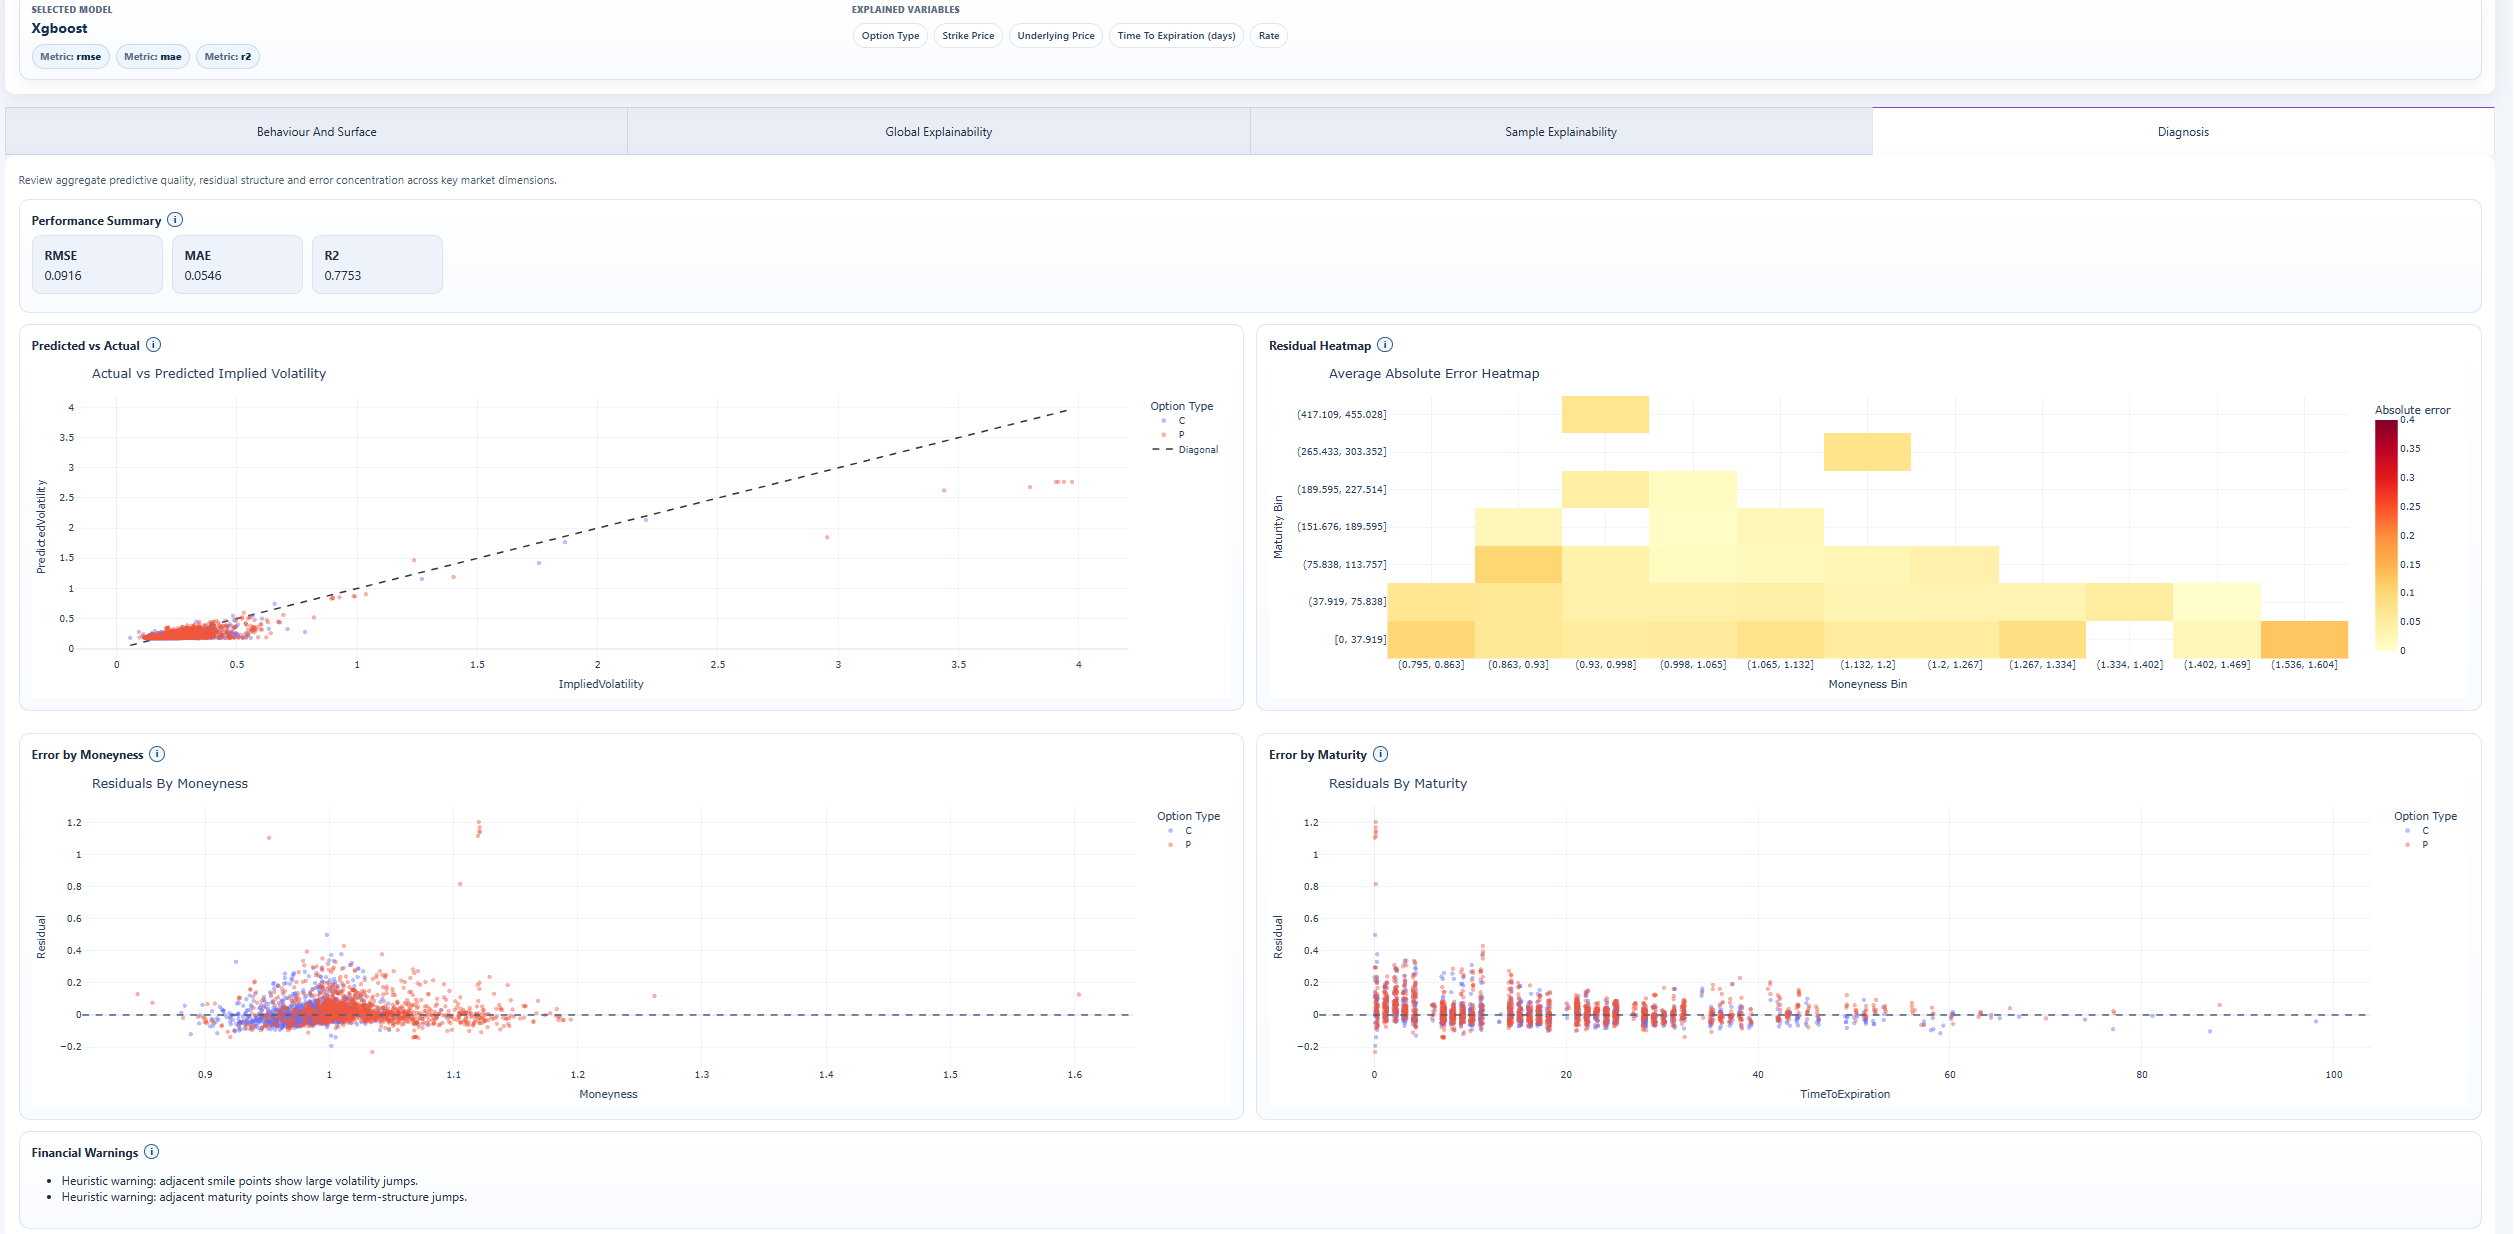
\includegraphics[width=\textwidth,height=0.24\textheight,keepaspectratio]{../imgs/dashboard/Diagnosis - Xgboost.png}
\caption*{\small \textbf{(a) XGBoost}}
\end{minipage}\hfill
\begin{minipage}{0.49\textwidth}
\centering
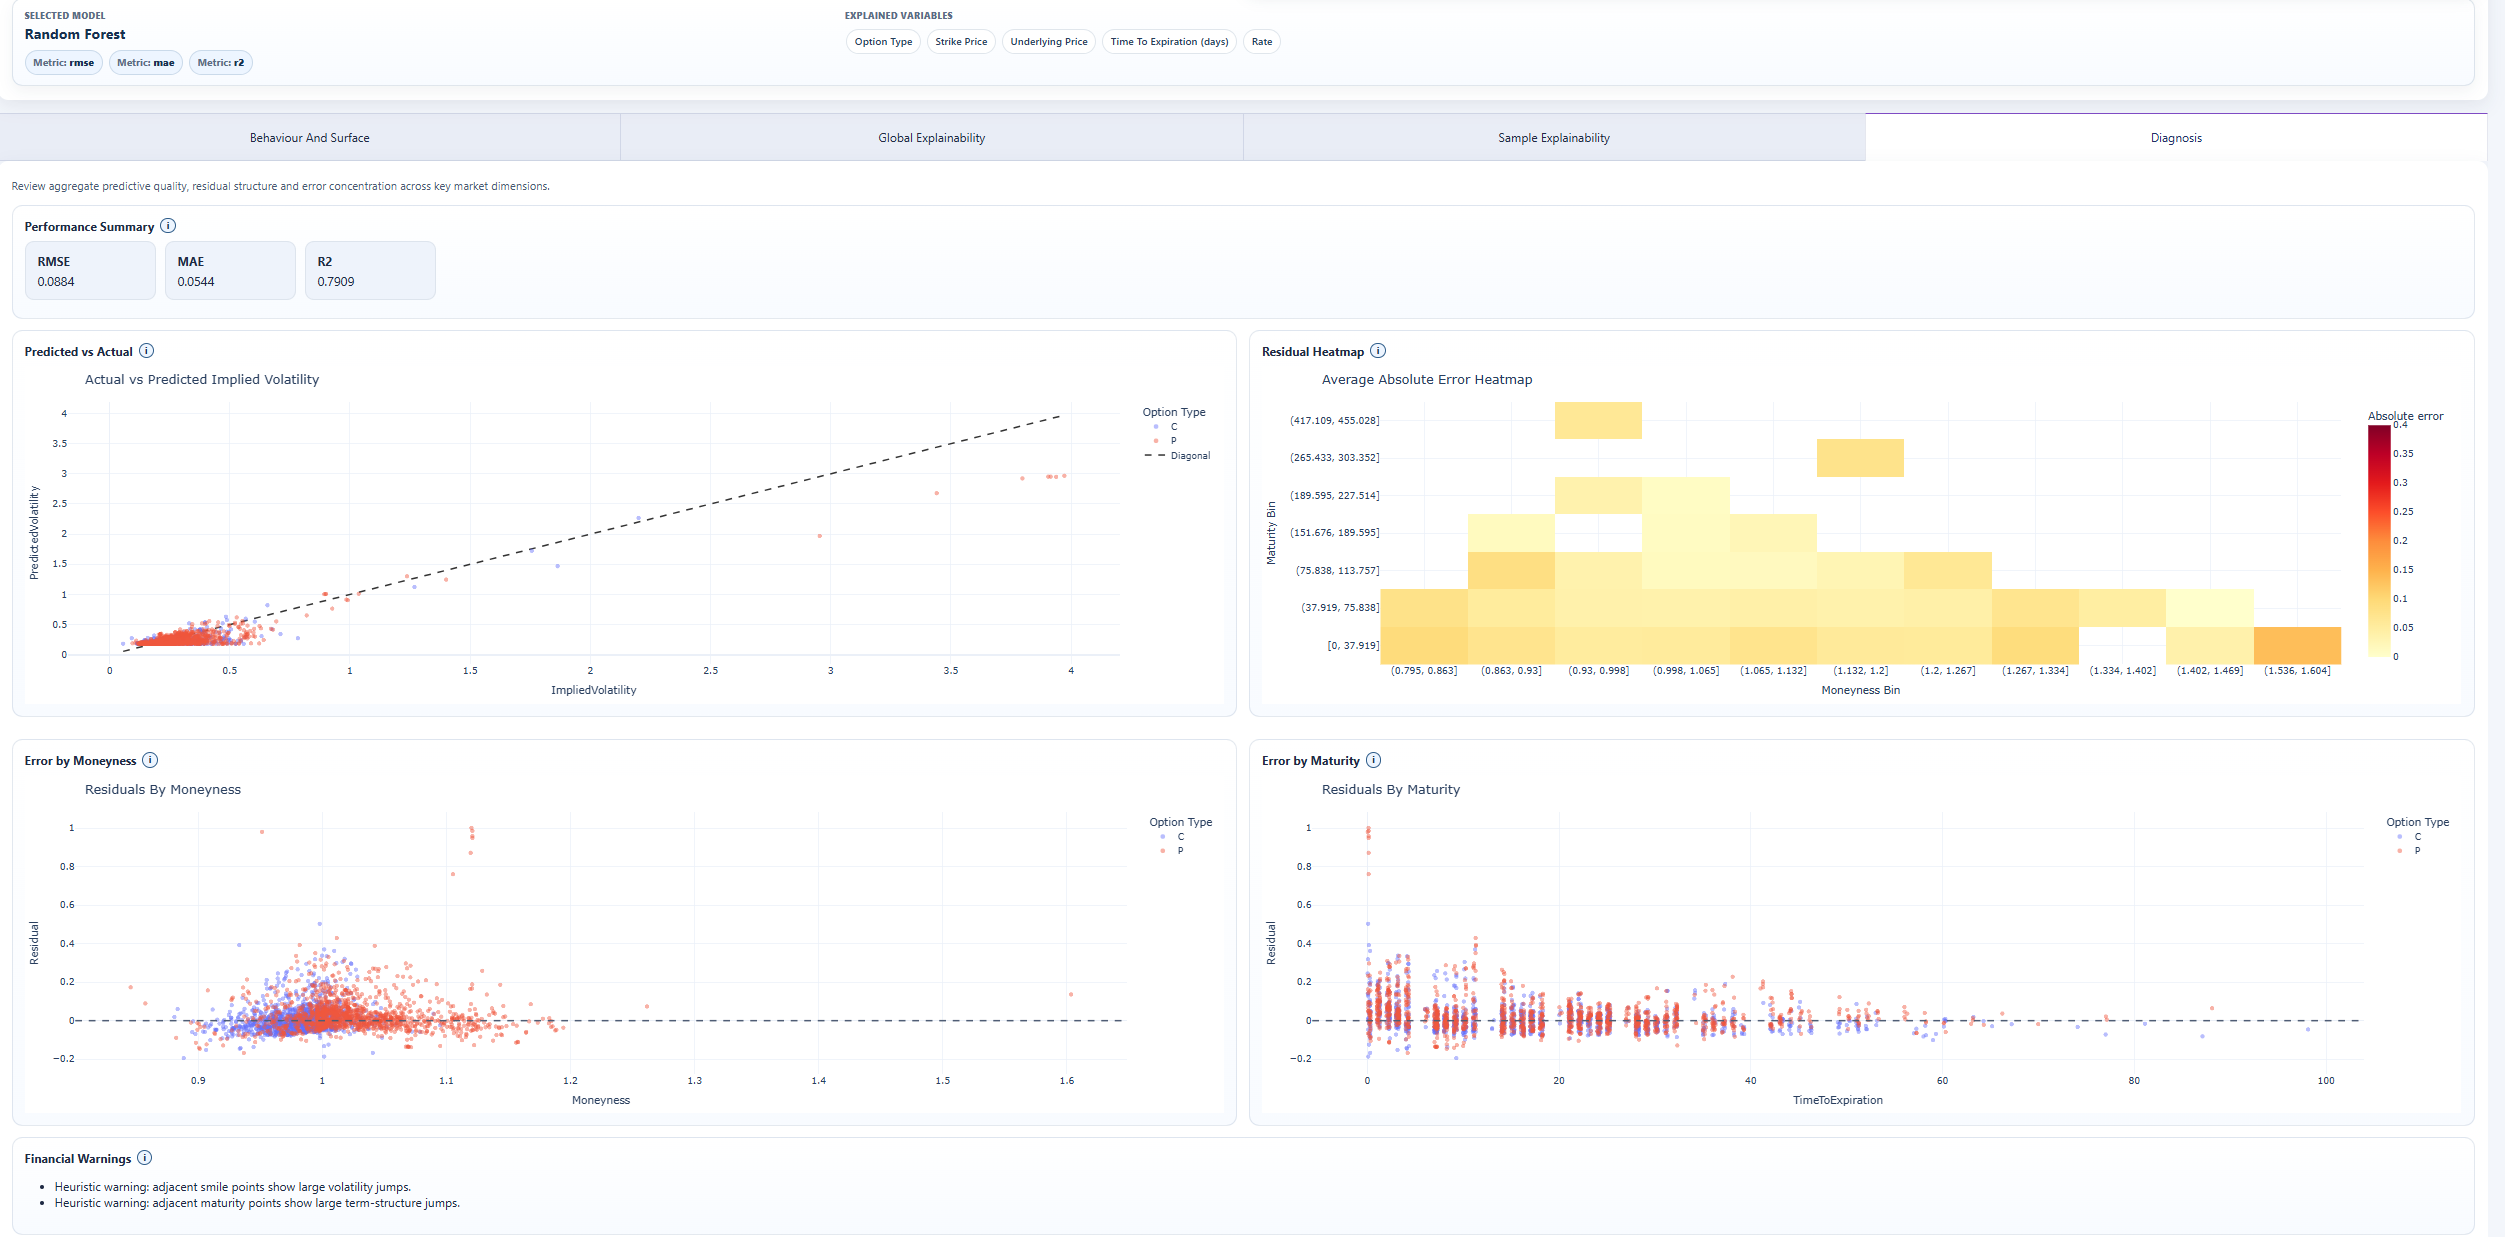
\includegraphics[width=\textwidth,height=0.24\textheight,keepaspectratio]{../imgs/dashboard/Diagnosis - Random Forest.png}
\caption*{\small \textbf{(b) Random Forest}}
\end{minipage}
\caption{\small Comparación de sensibilidad por moneyness y vencimiento: XGBoost versus Random Forest.}
\label{fig:app-sensitivity-rf-xgb}
\end{figure}

La Figura~\ref{fig:app-sensitivity-rf-xgb} permite una lectura directa por capas y comparación entre modelos. Primero, el \emph{Residual Heatmap} identifica si la concentración de error se desplaza hacia extremos de moneyness o hacia tramos de vencimiento concretos. Segundo, \emph{Error by Maturity} resume si los vencimientos cortos, medios o largos concentran más desviación. Tercero, \emph{Error by Moneyness} separa el desempeño entre regiones ITM, ATM y OTM. La comparación lado a lado revela que Random Forest (b) mantiene un patrón de error más estable y consistente respecto a XGBoost (a), con especial énfasis en la robustez en zonas extremas de moneyness. Si una zona presenta error estructuralmente mayor, esa zona requiere mayor prudencia en valoración, contraste adicional con modelos internos y monitorización reforzada de cobertura. En cambio, zonas con error bajo y patrón estable son candidatas a uso más sistemático del modelo como referencia de apoyo.
